%----------------------------------------------------------------------------
\chapter{Semantic models and parsing}
\label{chap:semanticparsing}
%----------------------------------------------------------------------------

In this chapter we first introduce applications, that use semantic models as an essential knowledge for their process. After, the theory and problems of semantic representation are discussed, and we briefly present the upsides and downsides of such representations. After that we go into details about distributional and graph based models, introducing the semantic parsing system \textbf{4lang}, which is the main focus of our work. Finally, our micro-services are discussed, built around the parser to highly automate the process of building concept graphs from raw input. An easy example of their usage is shown as well.

When we use the word semantics, we usually refer to the interpretation of a linguistics unit (e.g. words, phrases, sentences, or whole texts) within the boundaries of a certain context. In many scientific fields e.g. philosophy, logic or biology the study of semantics is a highly researched task. While many NLP tasks like syntactic parsing, part-of-speech tagging, or even machine translation can be ignorant of the meaning of units, of what information they hold, there are also many other tasks that rely heavily on semantics.

Some examples, where semantic analysis is unavoidable:
\begin{itemize}
	\item \textbf{Question answering} is the process of generating meaningful answers to the user's question, using some kind of knowledge. It might be considered one of the oldest tasks in NLP or in AI in general with machine translation. With the recent uprising products like Siri, Alexa, or Watson, it is still one of the most researched area.
	\item \textbf{Recognizing entailment} is whether a statement implies another or not, it is closely connected to \textbf{machine comprehension}, which is the main focus of our work.
	\item \textbf{Chatbots} are systems, that somewhat can simulate the conversation of humans.
	\item \textbf{Sentiment analysis} is the task of understanding the opinion about a subject. Usually can be considered as a classification problem, where in the simplest case two class, "\textit{negative}" and "\textit{positive}" is given. More complex version of the task is also present, where the detection of the target of the opinion is also the part of the problem. There are solutions for the problem with hand-crafted rules and machine learning algorithms as well.  
\end{itemize}

For modeling the meaning of linguistic units, choosing an appropriate representation of our model is needed. While for syntactic analysis widely accepted concepts and ideas (e.g. dependency tree, phrase structure trees) of such representation are already in use, for a semantic model it still remained a challenging task. Even answering the question \textit{"What is a semantic representation?"} is not well defined, and mostly decided by the nature of our task. The units of a semantic model are also not globally decided (word, phrase or a sentence?).

Finding an absolute representation of semantics knowledge is among the most difficult task in Artificial Intelligence (AI). While we are yet to find a representation that has no downside, various experimental models are present, that are applicable for certain domains, but are problematic in other scenarios. So before choosing one, we need to take into account the limitations of each choice. 


Representation of semantic knowledge with logical expressions (e.g. zero-order logic, prepositional logic) exists, and although many companies still rely on hand-crafted rules as a knowledge representation, they are very unpractical and have serious problems with scalability and automation. Distributional models have risen in popularity in recent years, where meaning is represented with multi-dimensional vectors. While vector based models can give us a uniform representation, they mostly lack interpretability in a way that we never really know what happens inside these models. Another issue is the choice of the dimension. Many algorithms exist for reducing the dimension of such vectors to a fixed number, but determining the correct length can be difficult. Rare words are a big issue as well, if a word in the training data is rarely present, distributional models will fail to handle them correctly.

On the other hand graph based solutions have high level of interpretability, and handling rare words is one of their biggest advantage. But automating the process of building graphs is a challenging task, and using them as a sole solution for a semantic parsing task in most cases would come short, but in hybrid systems they make up for the weaknesses other models have.

 In the next sections we will briefly discuss graph based models and distributional models, and because both of them have their merits, it is necessary to know the strengths and weaknesses of each one. Our work focuses around graph based solutions.

\section{Distributional model}
In the field of natural language processing one way of encoding semantic meaning is to use distributional models. In these models, two words are similar if they appear in the same context, and model semantic meaning as real-valued vectors. These vectors need to be constructed from a training data, and we can calculate similarity as cosine distance between the vectors.

Let's have a look at these two sentences \textit{"The cat is walking in the bedroom"} and \textit{"A dog was running in a room"}. Words \textit{"dog"} and \textit{"cat"} have a similar semantic meaning, so if they are represented by vectors, and their cosine distance from each other is small, then we can vary the sentences \textit{"The dog is walking in the bedroom"} and \textit{"A cat was running in a room"} \cite{Bengio:2003}. These models take surrounding words into account and their goal is to obtain the meaning of the target word from their surroundings\cite{Jurafsky:2018}, and because \textit{"dog"} and \textit{"cat"} are close in vector space, they most likely will appear in the same context. This intuition helps us generalize sentences. These meanings are represented by vectors, called embeddings. One of the first models built around these intuitions were introduced by Bengio \cite{Bengio:2003}. 

These word embeddings are used in basically all state-of-the art systems related to natural language processing applications. Mikolov \cite{Mikolov:2013c} showed that word embeddings can be applied for vector operations, like addition or subtraction, and these operations often result in meaningful representation. If we have example words "\textit{King}", "\textit{Man}", "\textit{Woman}", then the vector("King") - vector("Man") + vector("Woman") \ref{fig:vecs} will most likely result in vector that is close to vector("Queen") in the embedding space.

 While the usage of word embeddings brought an important breakthrough in modeling word meaning, applying them for bigger linguistics units like phrases, sentences or even whole text remained a difficult challenge even for nowadays. One of the biggest reasons for this is the additive aspect of these models: if we model A B C expression with vector v(A) + v(B) + v(C), then we represent "John killed Bill" and "Bill killed John" sentences in the same way. 

\begin{figure*}[h!]
	\centering
	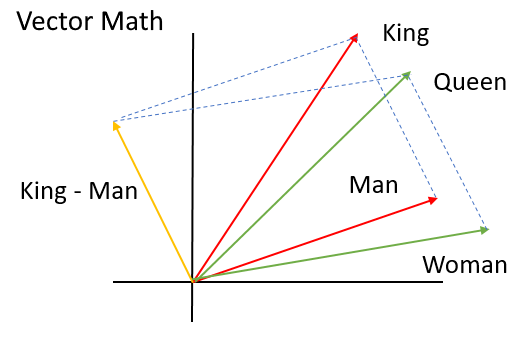
\includegraphics[width=0.7\textwidth]{figures/vecs}
	\caption{Vector addition example}
	\label{fig:vecs}
\end{figure*}

The other issue is that we know very little about the structure of a multi-dimensional real-value vectors (for embeddings it can be from 300 up to 1000 dimension), so this makes it very hard to understand their structure, and exactly in what scenario they work, and the reason when they don't. So while most state-of-the art systems use word embeddings as a sole representation of meaning, and while it can be useful to encode meaning as vectors, so it can create connection from language specific and non-language specific data, we cannot deny the importance of having other semantics representations, such as graph-based ones. 

In the majority of our work, we researched graph-based solutions, where we model the meaning of linguistics unit with graphs, and the whole process can be defined with graph transformations. Next I will briefly introduce graph based formalism starting with Abstract Meaning Representations (AMR) followed by the introduction of the \textbf{4lang} formalism, which will be the focus of the work, and I will go into details in the next section.

\section{Abstract Meaning Representations}
Abstract Meaning Representation (AMR) was introduced by Banarescu\cite{Banarescu:2013} for representing the meaning of linguistic structures. They represent meaning as directed acyclic graphs (DAGs), that can be used to capture the meaning of whole sentences, so if two sentences are similar in meaning, they should be represented by similar graphs. In the past few years, AMR related works have appeared e.g. parsing applications, or annotated corpuses \cite{Banarescu:2013, OGorman2018AMRBT, DAC:2017}.

Nodes of AMR graphs can be represented various ways. Each node in the graph represents a semantic concept \cite{AMR:2015}, that can be either an English word, or frameset from PropBank \cite{Palmer:2005}, essentially used for abstraction. The framesets are English verbs. The AMR introduced these variables for entities, events, properties, and states. An AMR can be converted to multiple formats:
\begin{itemize}
	\item Logic format
	\item AMR format
	\item Graph format
	
	These formats can be seen on Figure \ref{fig:amr} for sentence \textit{"the boy wants to go"}, and the corresponding 4lang representation on Figure \ref{fig:4langboy}.
	
\end{itemize}

\begin{figure*}[h!]
	\centering
	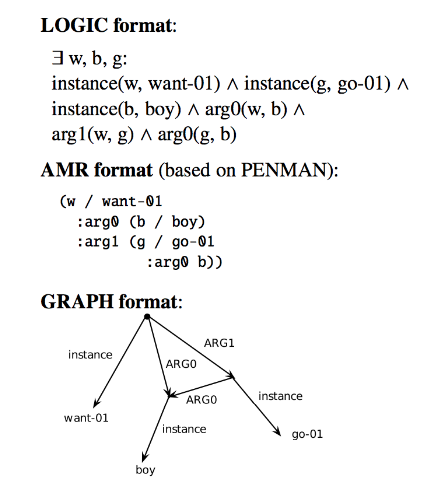
\includegraphics[height=0.4\textwidth]{figures/amr}
	\caption{Example sentence and representations}
	\label{fig:amr}
\end{figure*}

In this thesis we use the semantic parser \textbf{4lang} \cite{Recski:2015b}, and unlike \textbf{4lang}, AMR handles wider range of phenomenas, mostly typical of English. AMR's usage is mostly biased towards English \cite{Palmer:2005}, while 4lang can be configured to handle multiple languages.

\begin{figure*}[h!]
	\centering
	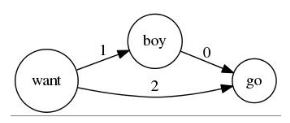
\includegraphics[width=0.3\textwidth]{figures/4langboy}
	\caption{Example sentence and representations in 4lang}
	\label{fig:4langboy}
\end{figure*}

In the next section, I will go into details about the \textbf{4lang} formalism, and the parser itself. After that I will describe our method of measuring similarities between semantic graphs, and it's usage on semantic related tasks.

%----------------------------------------------------------------------------
\section{4lang}
\label{sec:4lang}
%---
The \textbf{4lang} system is in the main focus of our work, in this section we will discuss the formalism and possible applications. \textbf{4lang} also means the manually built dictionary of mapping more than 2000 words to graphs, this is described in \cite{Kornai:2013}. After discussing the main formalism of \textbf{4lang}, we will demonstrate our highly automated process of building concept graphs, that was achieved by wrapping \textbf{4lang} functionality in micro-services building a REST-API, followed by our baseline for the machine comprehension task.

\subsection{The formalism}
The \texttt{4lang} system of semantic representation \cite{Kornai:2015a}
represents the meaning of linguistic units (both words and phrases)
as directed graphs of syntax-independent concepts. Every node of a \textbf{4lang} graph is a concept, which means that they are not taken as words, and they don't have any grammatical functions, like part-of-speech, voice, tense, etc.\cite{Recski:2016}.
Since these concepts have no grammatical attributes and no event structure, e.g.
the phrases \textit{water freezes} and \textit{frozen water} would both be
represented as \textit{water}~$\xrightarrow0$~\textit{freeze}. This also means that 4lang defines a many-to-one relation between the words and concepts. 

\textbf{4lang} formalism defines three types of edges:
\begin{itemize}
	\item \textbf{The 0-edge} represent represent attribution (\texttt{dog
		$\xrightarrow0$ large}), hypernymy (\texttt{dog $\xrightarrow0$ mammal}) and unary predication (\texttt{dog  $\xrightarrow0$ bark})
	\item \textbf{1- and 2-edges} those representing binary relations are connected to their arguments
	via edges labeled \texttt{1} and \texttt{2}, e.g \texttt{cat $\xleftarrow1$ catch $\xrightarrow2$ mouse}. Binaries that are shown with uppercase are binaries that must have two outgoing edges as shown in Figure \ref{fig:4langbin}. If we look at the sentence \textit{"Kinga broke Adam's bike"}, and the corresponding graph shown in Figure \ref{fig:4langbin}, if the 0-connection wouldn't be present between \textit{Kinga} $\xrightarrow0$ break, that would mean we consider that the relationship depend on whether the object of breaking is established or not. So in \textbf{4lang} the connection of 0-edge is present between a subject and a predicate regardless of the other arguments.
\end{itemize}

\begin{figure*}[h]
	\centering
	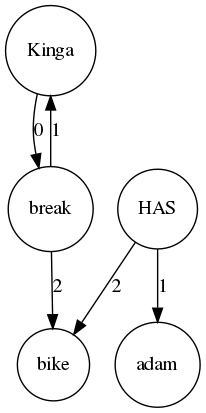
\includegraphics[height=0.5\textwidth]{figures/binary4lang}
	\caption{4lang with binaries}
	\label{fig:4langbin}
\end{figure*}

The example in
Figure~\ref{fig:bird} shows the \texttt{4lang} definition of the
concept \texttt{bird}. This definition was built manually, as part of
the \texttt{4lang} dictionary \cite{Kornai:2013}, but similar
definitions have been created automatically from definitions of
monolingual dictionaries such as Longman, using the
\texttt{dict\_to\_4lang} tool \cite{Recski:2016d}.

The open-source \textbf{4lang} pipeline\footnote{\url{https://github.com/kornai/4lang}}
contains tools for generating
directed graphs from raw text by mapping dependency edges in the output of the
Stanford parser \cite{deMarneffe:2006} to \texttt{4lang} subgraphs over
concepts corresponding to each word of the original sentence. The Stanford parser builds a dependency tree from the raw text that captures the syntactical relations between the linguistics units. \textbf{4lang} graph construction involves mapping from these relations to \textbf{4lang} semantics graphs, assigning the dependencies to \textbf{4lang} subgraphs. The mapping is presented in Table \ref{table:mapping}, and an example is shown for sentence \textit{"I like swimming"} in Figure \ref{fig:swimmingdep}, where we can see the dependency tree coming out of the Stanford parser, and the corresponding 4lang graph is present in Figure \ref{fig:swimming}, where the mapping from the dependency tree to \textbf{4lang} graph is done. 

\begin{table}
	\centering
	%\small
	\begin{tabular}{lc}
		\toprule
		Dependency & Edge \\
		\midrule
		amod & \multirow{7}{*}{\edge{$w_1$}{0}{$w_2$}} \\
		advmod & \\
		npadvmod & \\
		acomp & \\
		dep & \\
		num & \\
		prt & \\
		\midrule
		nsubj & \multirow{4}{*}{\twoedges{$w_1$}{1}{0}{$w_2$}} \\
		csubj & \\
		xsubj & \\
		agent & \\
		\midrule
		dobj & \multirow{6}{*}{\edge{$w_1$}{2}{$w_2$}} \\
		pobj & \\
		nsubjpass & \\
		csubjpass & \\
		pcomp & \\ 
		xcomp & \\
		\midrule
		appos & \twoedges{$w_1$}{0}{0}{$w_2$} \\
		\midrule
		poss & \multirow{2}{*}{$w_2\xleftarrow1$ \texttt{HAS} $\xrightarrow2w_1$} \\
		prep\_of & \\
		\midrule
		tmod & $w_1\xleftarrow1$ \texttt{AT} $\xrightarrow2w_2$ \\
		\midrule
		prep\_with & $w_1\xleftarrow1$ \texttt{INSTRUMENT} $\xrightarrow2w_2$ \\
		\midrule
		prep\_without & $w_1\xleftarrow1$ \texttt{LACK} $\xrightarrow2w_2$ \\
		\midrule
		prep\_P & $w_1\xleftarrow1$ \texttt{P} $\xrightarrow2w_2$ \\
		\bottomrule
	\end{tabular}
	\caption{Mapping from Stanford dependency relations to 4lang subgraphs \cite[p. 12.]{Recski:2018}.}
	\label{table:mapping}
\end{table}

\begin{figure*}[h]
	\centering
	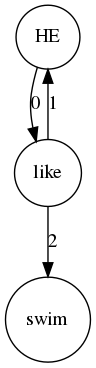
\includegraphics[height=0.5\textwidth]{figures/swimming}
	\caption{4lang example of a sentence}
	\label{fig:swimming}
\end{figure*}

\begin{figure*}[h]
	\centering
	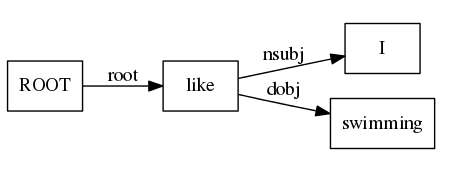
\includegraphics[width=0.5\textwidth]{figures/swimmingdep}
	\caption{Stanford example of a sentence}
	\label{fig:swimmingdep}
\end{figure*}


\subsection{Expansion}
Optionally, the \texttt{4lang} system allows us to \textit{expand}
graphs, a process which unifies the graph with the definition graphs of
each concept. The implementation is written in the \textbf{dict\_to\_4lang} module, that extends the functionality of the discussed \textbf{text\_to\_4lang} pipeline with dictionaries. \textbf{4lang} takes advantage of this, and implements the expansion step, which essentially is joining the definitions graphs to the main graph. This allows us to build a larger graph, that contains more information, and allows us to model the text better by simply adding the definition of words.

Let us look at the example sentence \textit{"My poor wife"}, that results the graph shown in Figure \ref{fig:mypoor}. Looking at the definition of the word \textit{poor}: \textit{having very little money and not many possessions}, we can build a definition graph and essentially join the two graphs together. This can result us a better model if we are ready to take word definitions into account, and with this method we can have higher similarities between graphs whose sentences are also similar. Doing this for every word in the sentence resulting in a merged graph Figure \ref{fig:mypoorexpanded}. If we look at the graph, it is clear that the expanded graph gives us much more accurate context and definition. Our work was build around the expanded graph, and we will see that how better it actually performs on a real task. This will be the main topic of the next chapter.

\begin{figure}
	\centering
	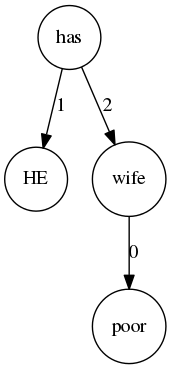
\includegraphics[scale=0.5]{figures/mypoor}
	\caption{4lang definition of sentence \textit{"My poor wife"}.}
	\label{fig:mypoor}
\end{figure}

\begin{figure}
	\centering
	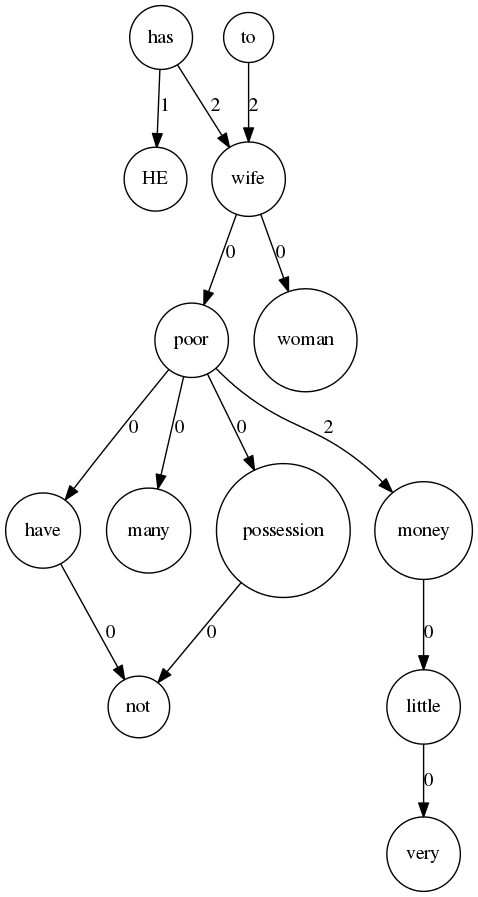
\includegraphics[scale=0.5]{figures/mypoorexpanded}
	\caption{4lang definition of expanded sentence \textit{"My poor wife"}.}
	\label{fig:mypoorexpanded}
\end{figure}


\subsection{The service}
The beginning of our research we put a high emphasis on generating graphs from raw text with a highly automated method, so besides being an open-source software library,
the \texttt{4lang} we made the accessible via a public
REST API at \url{http://hlt.bme.hu/4lang}. We used the python language for implementing the service, and for the framework we used the flask\footnote{http://flask.pocoo.org/} package. The service generates input for the \texttt{text\_to\_4lang} module from the raw text input, then after processing it, returns a graph in \textbf{networkx multigraph}\footnote{\url{https://networkx.github.io/documentation/networkx-1.9.1/reference/classes.multigraph.html}} format to make it easy to visualize it on essentially any client side. The process is as easy as follows:
\begin{center}
	\begin{lstlisting}
sentence = "I like micro-services." 
data = {'sentence':   sentence}
data_json = json.dumps(data)
payload = {'json_payload': data_json}
headers = {'Content-type': 'application/json', 'Accept': 'text/plain'}
r = requests.post("http://hlt.bme.hu/4lang/sendef", 
data=data_json, headers=headers)
s_machines = r.json()['sentence']
\end{lstlisting}
\end{center}


The generated graph can be seen in Figure \ref{fig:service}. The code of the service is publicly available on Github\footnote{\url{https://github.com/adaamko/4lang}}. We can generate graphs with raw text by calling the service. Currently our service has multiple endpoints, with each of them representing different methods.
If you are interested in only processing a single sentence, the following endpoints are available:

\begin{figure}[!htb]
	\centering
	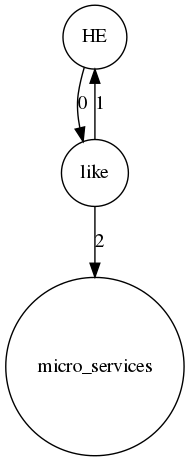
\includegraphics[scale=0.5]{figures/service}
	\caption{4lang definition of sentence \textit{"I like micro-services"}.}
	\label{fig:service}
\end{figure}

\begin{itemize}
	\item \textbf{/sendef} - Returns the graphs built from the sentence.
	\item \textbf{/senexp} - Returns the graphs, where the word's definition has been added to the graph.
	\item \textbf{/senabs} - Calling this function, we defined some rules, where we can build a more abstract graph using the definitions, this is more of a future work, I will briefly mention the algorithms and ideas behind it in the last chapter.
\end{itemize}
You can get a word's definition by calling the defined endpoint:
\begin{itemize}
	\item \textbf{/definition} - Returns the graphs built from the word's definition.
\end{itemize}
For the machine comprehension task we defined a dedicated endpoint:
\begin{itemize}
	\item \textbf{/rally} - Returns a merged graph, where we merge a question sentence with an answer sentence. The main goal of this endpoint is that we can get a graph that can be explicitly compared with graph built from the passage text (it will be explained in the next chapter in details). 
\end{itemize}


\begin{figure}[!htb]
	\centering
	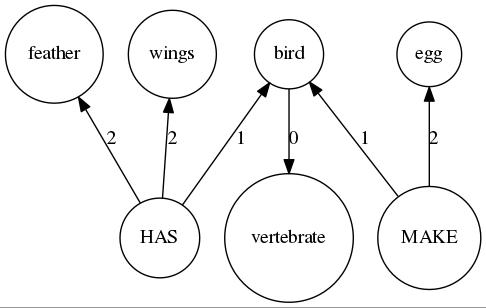
\includegraphics[scale=0.5]{figures/bird}
	\caption{4lang definition of \texttt{bird}.}
	\label{fig:bird}
\end{figure}

Graphs generated by the \texttt{4lang} parser have previously been used
successfully in measuring semantic similarity. The current state of the
art system on the \texttt{SimLex-999} benchmark \cite{Hill:2014a}
outperforms previous top systems by utilizing a simple similarity metric
between \texttt{4lang} definitions of pairs of English words
\cite{Recski:2016c}, this was the main idea of trying it in a different task with a different state-of-the-art system.

In the next chapter, I will briefly discuss the machine comprehension challenge, and I will introduce our baseline method for solving it using our micro-service for automatically build concept graphs. After that we will present how it is applicable to an already working system.